\section{Optimal Control of Pitch and Travel without Feedback}\label{sec:prob2}

In this section an optimal trajectory $x^*$ and a corresponding input sequence $u^*$ was calculated. The trajectory should bring the helicopter from an initial state to another predefined state. No feedback was used to correct for deviations from the calculated trajectory. Also, elevation was disregarded, that is, $e=0$ was assumed for this part. The computation of the optimal trajectory was formulated as a discrete convex optimization problem.


\subsection{The helicopter model on continuous-time state-space form}

The system (\ref{eq:model_al}) describes the helicopter plant, with a basic control layer consisting of PID and PD controllers for elevation and pitch. The optimization layer gives the inputs to these regulators, as shown in figure (\ref{fig:control_hierarchy}).

\begin{figure}[ht]
	\centering
	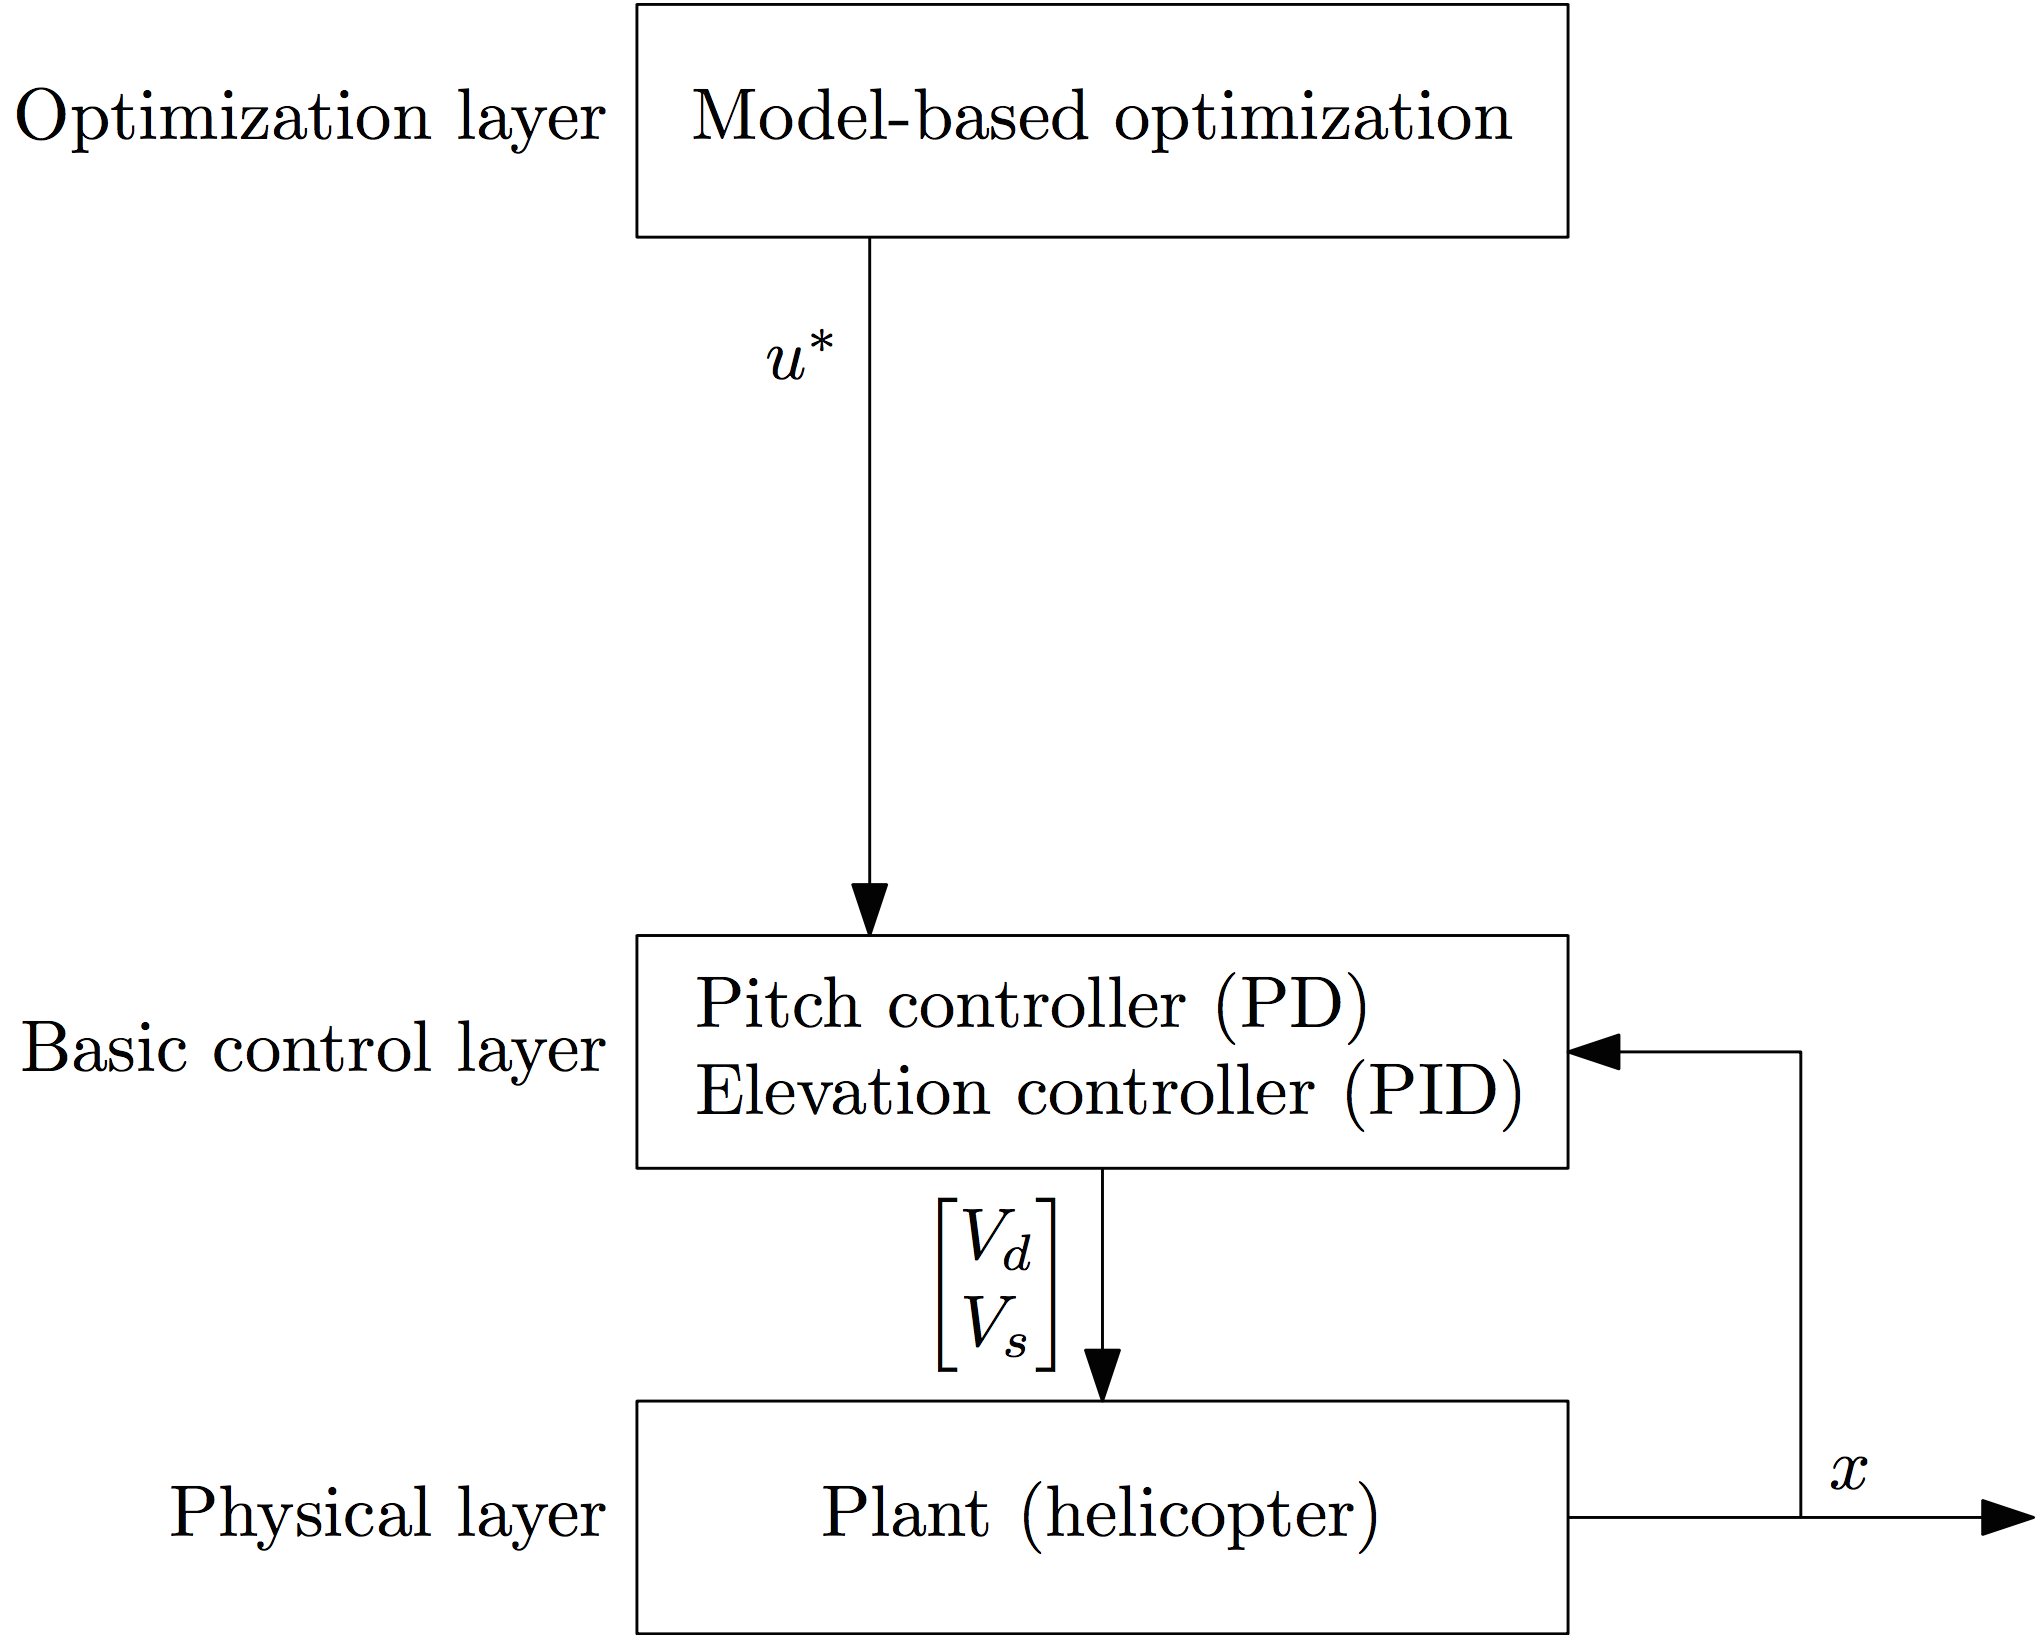
\includegraphics[width=0.6\textwidth]{figures/day2/control_hierarchy_day2}
	\caption{Control hierarchy}
	\label{fig:control_hierarchy}
\end{figure}

The system can be written on continuous-time state-space form:

\begin{equation}
    \dot{x} = A_cx + B_cu
    \label{eq:state_space_axbu}
\end{equation}

with $x = \begin{bmatrix} \lambda & r & p & \dot{p} \end{bmatrix}^T$ and $u = p_c$.
The continuous-time system matrices for this model are:

\begin{equation}
	A_c = \begin{bmatrix} 0 & 1 & 0 & 0 \\ 0 & 0 & -K_2 & 0 \\ 0 & 0 & 0 & 1 \\ 0 & 0 & -K_1K_{pp} & -K_1K_{pd} \end{bmatrix}
	\qquad\text{and}\qquad
	B_c = \begin{bmatrix}0 \\ 0 \\ 0 \\K_1K_{pp} \end{bmatrix}
\end{equation}


\subsection{Discretization}

The system dynamics was implemented as a sequence of constraints in the optimization problem, and the system model therefore had to be written in discrete-time state-space form,

\begin{equation}
	x_{k+1} = Ax_k + Bu_k.
	\label{eq:discrete_state_space_axbu}
\end{equation}

The model was discretized using the Forward-Euler method with timestep $h$.

\begin{equation}
	\dot{x}_k \approx \frac{x_{k+1} - x_k}{h}
\end{equation}

Inserting this into (\ref{eq:state_space_axbu}),

\begin{equation}
	\dot{x}_{k+1} \approx (I + hA_c) x_k + hB_c u_k
\end{equation}

is obtained. A suitable approximation for the discrete-time matrices is then

\begin{equation}
	A \approx I + hA_c
	\qquad\text{and}\qquad
	B \approx hB_c
\end{equation}

These matrices were computed in Matlab, and are therefore not shown explicitly here.


\subsection{Computation of optimal trajectory}

An optimal trajectory can be generated by minimizing the cost function

\begin{equation}
	\label{eq:trajectory_cost}
	\phi = \sum_{i=1}^{N}(\lambda_i - \lambda_f)^2 + qp_{ci}^2
\end{equation}

for some scalar weight $q \geq 0$ over the finite horizon of states and inputs

\begin{equation}
	z = (x_1 \; x_2 \; ... \; x_N \; u_1 \; u_2 \; ... \; u_N)^T
\end{equation}

This was done in Matlab using the function quadprog. The discrete system dynamics was implemented as equality constraints of the form $A_{\text{eq}}z = B_{\text{eq}}$, where $A_{\text{eq}}$ and $B_{\text{eq}}$ are given by the left- and right-hand side of the $N$ constraints

\begin{align*}
	x_1 - Bu_0        &= Ax_0 \\
	x_2 - Ax_1 - Bu_1 &= 0    \\
	\vdots                    \\
	x_N - Ax_{N-1} - Bu_{N-1} &= 0
\end{align*}

We would also like to constrain the system state and input to be within a range

\begin{align}
	x^{\text{min}} \leq x_{t+1} \leq x^{\text{max}} \\
	u^{\text{min}} \leq u_t \leq u^{\text{max}}
\end{align}

for $t = 0...N-1$. Applying these constraints to all states and inputs in the solution horizon, we have

\begin{equation}
	\begin{bmatrix} I \\ -I \end{bmatrix} z
	\leq
	\begin{bmatrix}
	\{x_{t+1}^{max}\} \\
	\{u_t^{max}\} \\
	\{x_{t+1}^{min}\} \\
	\{u_t^{min}\}
	\end{bmatrix}_{t=0..N-1}
\end{equation},

which can be implemented as an inequality constraint of the form $A_{\text{iq}} z \leq B_{\text{iq}}$. Solving the optimization problem with different weights $q$ did not lead to any significant differences in the trajectory, this because the model inaccuracies made the helicopter drift away from the desired state anyway.

The objective function (\ref{eq:trajectory_cost}) weights %er dette riktig ord for å vekte noe?
the input relative to the state deviations using the weight parameter $q$. The term $(\lambda_i - \lambda_f)^2$ is the state deviations. They are squared to prioritize the largest deviation. Note that the cost function (\ref{eq:trajectory_cost}) does not take into consideration that $\lambda_i$ plus some multiple of $2\pi$ describes the same physical orientation of the helicopter. For example, if the reference is $0$ and $\lambda_i = 2\pi$, it will be regarded as a large error, even though the helicopter is in fact in the desired orientation. A more optimal scheme would take this into consideration.


\subsection{Implementation}

Figure (\ref{fig:day2_plot}) shows the implementation with $q = 1$. Zeroes were added on both sides of the input sequence to give time to initialize and stabilize the helicopter. As can be seen from the figure, the helicopter does not reach its desired final state. 

\begin{figure}[htb]
	\centering
   		\makebox[\textwidth][c]{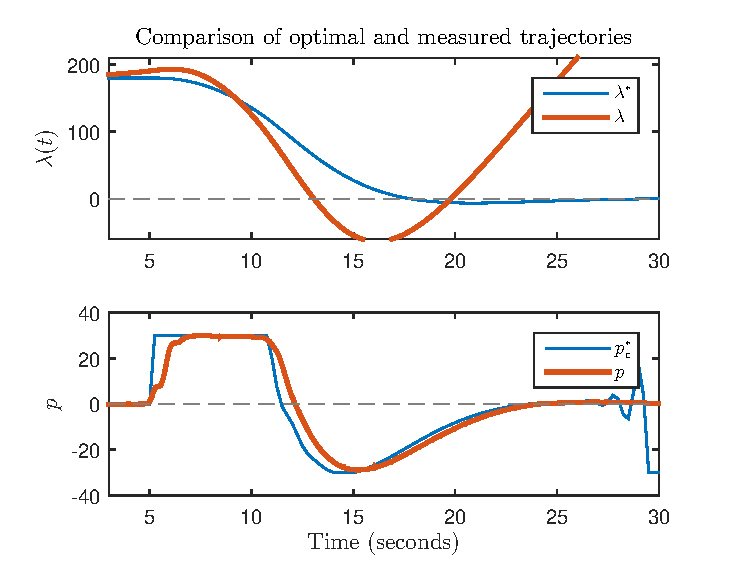
\includegraphics[width=\textwidth]{figures/day2/plot_day2}}
	\caption{Plot of day 2}
	\label{fig:day2_plot}
\end{figure}

The deviation was caused by an imperfect model. A perfect model is  unrealistic to construct, and without feedback, the model inaccuracies will lead to nonoptimal results in the real world. For example, the pitch-regulator in our model is fast enough to follow its input perfectly, and we are using a linear model that clearly does not correspond perfectly to the real helicopter.